\documentclass[ChapterTOCs,krantz2]{krantz} % Use krantz2 for 7" x 10" trim size
\usepackage{graphicx}
\usepackage{subfigure}
\usepackage{epigraph}
%-----------------------------------------------------------------------------
% Special-purpose color definitions (dark enough to print OK in black and white)
\usepackage{color}

% A few colors to replace the defaults for certain link types
\definecolor{orange}{cmyk}{0,0.4,0.8,0.2}
\definecolor{darkorange}{rgb}{.71,0.21,0.01}
\definecolor{darkgreen}{rgb}{.12,.54,.11}

%-----------------------------------------------------------------------------
% The hyperref package gives us a pdf with properly built
% internal navigation ('pdf bookmarks' for the table of contents,
% internal cross-reference links, web links for URLs, etc.)
%\usepackage{hyperref}

\usepackage{url}

%% Define a new 'leo' style for the package that will use a smaller font.
\makeatletter
\def\url@leostyle{%
  \@ifundefined{selectfont}{\def\UrlFont{\sf}}{\def\UrlFont{\small\ttfamily}}}
\makeatother
%% Now actually use the newly defined style.
\urlstyle{leo}

%\newcommand{\asterism}{{ \footnotesize \smash{% 
%    \raisebox{-.2ex}{% 
%      \setlength{\tabcolsep}{0.5pt}%
%      \begin{tabular}{@{}cc@{}}% 
%  \multicolumn2c*\\[-1.5ex] *&*% 
%\end{tabular}}}}}

\newcommand{\parasep}{\begin{center}*\hspace{6em}*\hspace{6em}*\end{center}}

\newcommand*{\threesim}{%
 \mathrel{\vcenter{\offinterlineskip
  \hbox{$\sim$}\vskip-.35ex\hbox{$\sim$}\vskip-.35ex\hbox{$\sim$}}}}

\newcommand{\asterism}{\smash{%
  \raisebox{-.5ex}{%
    \setlength{\tabcolsep}{-.5pt}%
    \begin{tabular}{@{}cc@{}%
  \multicolumn2c*\\[-2ex]*&*%
\end{tabular}}}}}

%-----------------------------------------------------------------------------
%
% Commands for annotating the docs with fixme and inter-author notes.  See
% below for how to disable these.
%
% Define a \fixme command to mark visually things needing fixing in the draft,
% as well as similar commands for each author to leave initialed special
% comments in the document.
% For final printing or to simply disable these bright warnings, copy
% (there's a target macros_off' in the makefile that does this) the file
% macros_off.tex to macros.tex
\usepackage{amssymb}

\newcommand{\fix}[1] { \textcolor{red} {
{\fbox{ {\bf Fix:} \ensuremath{\blacktriangleright }} {\bf #1}
\fbox{\ensuremath{\blacktriangleleft} } } } }

% And similarly, one (less jarring, with fewer symbols and no boldface) command
% for each one of us to leave comments in the main text.
\newcommand{\fperez}[1] { \textcolor{blue} {
\ensuremath{\blacklozenge} {\bf fperez:}  {#1}
\ensuremath{\blacklozenge} } }

\newcommand{\jarrod}[1] { \textcolor{darkgreen} {
\ensuremath{\bigstar} {\bf jarrod:}  {#1}
\ensuremath{\bigstar} } }

\newcommand{\mref}[1] { \textcolor{darkorange} {
\ensuremath{\blacksquare} {\bf missing ref:}  {#1}
\ensuremath{\blacksquare} } }

%% Uncomment these to turn all the special marker commands off
%\renewcommand{\fix}[1]{}
%\renewcommand{\fperez}[1]{}
%\renewcommand{\jarrod}[1]{}
%\renewcommand{\mref}[1]{}

\begin{document}

\title{Dummy title}
\author{Dummy author}
\chapter*{Dummy chapter needed for the \textbackslash chapterauthor command to work later}

\mainmatter

\chapterauthor{Fernando P\'{e}rez}{Henry H. Wheeler Jr. Brain Imaging Center\\
Helen Wills Neuroscience Institute\\
University of California, Berkeley}
\chapterauthor{K. Jarrod Millman}{Division of Biostatistics\\
School of Public Health\\
University of California, Berkeley}


\chapter{Two cultures: open source software and scientific research}

As members of both the scientific research and the open-source
software development communities, we have observed that the latter
often lives up better than the former to our ideals of scientific
openness and reproducibility.  We explore the reasons behind this,
and argue that these problems are particularly acute in computational
domains where they should be in fact less prevalent.   We discuss
how we can draw specific lessons from the open source community both
in terms of technical approaches and of changing the structure of
incentives, to make progress towards a more solid base for reproducible
computational research.

\section{Introduction}\label{intro}

\setlength{\epigraphrule}{0pt}
\setlength{\epigraphwidth}{.65\textwidth}
\epigraph%
{%
  Science alone of all the subjects contains within itself the lesson of the
  danger of belief in the infallibility of the greatest teachers in the
  preceding generation\ldots Learn from science that you must doubt the experts.
}%
{\textit{What is Science? (1969)}\\ \textsc{Richard Feynman} }

Scientific research has become pervasively computational. In addition
to experiment and theory, the notions of simulation and data-intensive
discovery have emerged as third and fourth pillars of science \cite{4th-paradigm}.
Today, even theory and experiment are computational, as virtually
all experimental work requires computing (whether in data collection,
pre-processing or analysis) and most theoretical work requires symbolic
and numerical computing to develop and refine models. Scanning the pages
of any major scientific journal, one is hard-pressed to find a publication
in any discipline that doesn't depend on computing for its findings.

And yet, for all its importance, computing is often treated as an
afterthought both in the training of new scientists and in the conduct
of everyday research. Most working scientists have witnessed how computing
is treated as a task of secondary importance that students and postdocs
learn ``on the go'' with little training to ensure that results
are trustworthy, comprehensible and ultimately a secure foundation
for reproducible outcomes. Software and data are stored with poor
organization, documentation and tests. A patchwork of software tools
is used with limited attention paid to capturing the complex workflows
that emerge, and the evolution of code is often not tracked over time,
making it difficult to understand how a result was obtained. Finally,
many of the software packages used by scientists in research are proprietary
and closed-source, preventing the community from having a complete
understanding of the final scientific results.

\subsection{Growing crisis}

The situation above will be familiar to all scientists and this familiarity
may breed complacency. However, the consequences of this situation are serious
at present and will become disastrous if the situation is not dealt with
directly. 

Much more than a ``third branch'' of science, computing has become so central
to scientific practice that it is almost unimaginable to find a working
scientist that could claim the don't use computers at all.  Experimentalist
from biology to physics and observationalist from astronomy to climate study
are confronted with an avalanche of quantitative data.  All scientists must now
do real computing.  As computers continue to increase in computational power and
storage capacity, the problems only compound.  While better computing practices
won't directly translate to better science, current practices do lead to bad
science.

Consider, just to name two widely publicized cases, the loss of public
confidence in the``Climategate'' fiasco \cite{Hef10} or the Duke cancer trials
scandal, where sloppy computational practices likely led to severe health
consequences for several patients \cite{Cou10}. 

The situation is more common than we'd like to believe:
\begin{itemize}
\item Begley \& Ellis, Nature, 3/28/12: {\emph Drug development:
Raise standards for preclinical cancer research.}
\item 47 out of 53 ``landmark papers'' could not be replicated.
\end{itemize}
See Nature, Feb 2012, Ince et al: {\emph The case for open computer programs}
\begin{itemize}
\item The scientific community places more faith in computation
than is justified
\item anything less than the release of actual source code is an
indefensible approach for any scientific results that depend on computation
\end{itemize}


The ability to reproduce and verify results is a hallmark of the
scientific method.

A crisis of credibility and real issues

Retraction rates are going up \cite{cokol2008retraction,steen2011retractions} 
\subsection{Contrast of cultures}

Open source software development uses public fora for most discussion
and systems for sharing code and data that are powerful
provenance tracking systems. There is a strong culture of public disclosure,
tracking and fixing of bugs, and development often includes exhaustive
validation tests that are executed automatically whenever changes
are made to the software and whose output is publicly available on
the internet. This helps with early detection of problems, mitigates
their recurrence, and ensures that the state and quality of the software
is a known quantity under a wide variety of situations (operating
systems, inputs, parameter ranges, etc). Additionally, the same systems
that are used for sharing the code track the authorship of contributions.
All of this ensures that open collaboration does not dilute the merit
or recognition of any individual developer, and allows for a meritocracy
of contributors to develop while enabling highly effective collaboration.

In contrast, the incentives in scientific research are strongly
biased towards the rapid publication of novel results without any serious
requirement of validation. The outcome is that results from publications
in computationally-based research, which means essentially any type of
scientific research, are often impossible to reproduce. Sometimes
this is due to the code not being available at all in the first place.
Authors often do make codes available---thus fulfilling a token requirement
of disclosure---but in such a state that this disclosure is not a
practical solution to the reproducibility problem. A static archive
of source code that has never been tested in a computer or operating
system outside of the author's, never been audited by external eyes
and with no automatic testing built into it, is highly unlikely to
work reliably when used in a completely new environment.

\subsection{Pragmatic approach}

Notwithstanding the above, there are real issues with attempting to
naively transplant the practices of open source development directly
to computational research. The open source model ends up being one
where, in practice, the copyright and authorship of any large collaborative
project is spread among many authors, possibly thousands. While
the source control tools in use do allow for a relatively precise
provenance analysis to be performed if desired, this is rarely done
and its success is contingent on the community having followed certain
steps rigorously to ensure that attribution was correctly recorded
during development.

This is not a major issue in open source, as the rewards mechanisms
tend to be more informal and based on the overall recognition of any
one contributor in the community. Sometimes people contribute to open
source projects as part of their official work responsibilities, and
in that case a company can enact whatever policies it deems necessary;
often contributions are made by volunteers for whom an acknowledgment
in the project's credits is sufficient recognition.

In contrast, the academic world overwhelmingly weighs the authorship
of scholarly articles and conference proceedings as the main driver
of all forms of professional advancement and reward. In this system,
the pecking order of authorship matters enormously (with the many
unpleasant consequences familiar to all of us), and so does the total
number of authors in a publication. While in certain communities papers
with thousands of authors do exist (experimental high-energy physics
being the classic example), most scientists need the prominent visibility
they can achieve in a short author list. The dilution of authorship
results from a largely open collaborative development model
is an important issue that must be addressed.

Furthermore, the notion of a fully open development model typical
of open source projects is at odds with another aspect of the
scientific publication and reward system: the ``first
to publish'' race. Many scientists are, understandably,
be leery of exposing their projects on an openly accessible website
when in their embryonic stages. The fear of being scooped by others
is very real, and again we must properly address it as we consider
how to apply the lessons of open source development to the scientific
context.


\subsection{Limits of reproducibility}

As we seek to learn how the open source practice can inform our scientific
work, we must recognize that the ideal of scientific reproducibility
is by necessity a reality of shades. We can see a gradation that goes
from a pure mathematical result whose proof should be accessible to
any person skilled in the necessary specialty, to one-of-a-kind experiments
such as the Large Hadron Collider or the Hubble Space Telescope, that
can't be reproduced in any realistic sense. At each point in this
spectrum, however, we can always find ways to improve our confidence
in the results: whether we re-analyze the same unique datasets with
independently developed packages run by separate groups or we re-acquire
partial sampling of critical data multiple times, we should never
completely renounce the ideals of reproducibility because of practical
difficulties.

Similarly, in computational research we also have certain areas where
complete reproducibility is more challenging than others. Some projects
require computations carried on the largest supercomputers on the
planet, and these are very expensive resources that can't be arbitrarily
allocated for repeated executions of the same problem. Others may
require access to enormous datasets that can't easily be transferred
to the desktop of any researcher wishing to re-execute an analysis.
But again, alternatives exist: it should be possible to validate scaled
versions of the largest problems run independently, against scaled
specimens created on the supercomputers for this very purpose, and
sub-sampled datasets can be used to collect at least validation statistics
that may be informative of the trust we place on the published analysis.

\begin{itemize}
\item Levels of reproducibility: replication, validation, reproduction,
new construction.
\item Conditions: clarity, transparency and trace-ability, predictability
(which requires automation), communicability
\end{itemize}

While the mechanical reproduction of computational results is not a
panacea in itself; the rigor, openness, culture of validation, collaboration and
other aspects of science must become a routine part of our computational practices.

\parasep

In the next section, we share lessons we've learned from our participation in
several open source development projects and describe how these lessons can be
applied to scientific practice.  In the following section, we present a
comprehensive view of the role computing plays in the life-cycle of scientific
investigation.  In addition to surveying the standard approaches, this section
ends with a detailed overview of the open source IPython project
\cite{PER-GRA:2007}, which is a single software tool capable of spanning the
entire life-cycle of computational research.  Finally, we conclude with a brief
discussion of how we see the culture changing and the need for reviewing our
current incentive models and the training of new scientists.

\section{Lessons from open source}\label{lessons-oss}

Over the last decade, we've had the privilege of participating in a loose-knit
community of scientists, researchers, and engineers working to create a powerful
stack of open source tools for scientific computing written in Python.  Among
high-level open source programming languages, Python is today the leading tool
for general-purpose scientific computing (along with R for statistics),
finding wide adoption across research disciplines, education and industry and
being a core infrastructure tool at institutions such as CERN and the Hubble
Space Telescope Science Institute
\cite{millman2011python,Perez2011,ganga09,SST}.


core tools: numpy, scipy, matplotlib, and ipython

- simultaneously we've interacted heavily with researchers in
physics, psychology, neuroscience, and medicine.

- we've also talked with members of SciPy community representing
other disciplines and 


\subsection{Two cultures}

In his influential 1959 Rede Lecture, C. P. Snow lamented the separation between the
two cultures of science and humanities.  In particular, he warned that a lack
of understanding of scientific ideas among the intellectual classes was a major
impediment to solving the problems of modern society \cite{snow1960two}.

\begin{quote}
A good many times I have been present at gatherings of people who, by the
standards of the traditional culture, are thought highly educated and who have
with considerable gusto been expressing their incredulity at the illiteracy of
scientists. Once or twice I have been provoked and have asked the company how
many of them could describe the Second Law of Thermodynamics. The response was
cold: it was also negative. Yet I was asking something which is about the
scientific equivalent of: Have you read a work of Shakespeare’s?
\end{quote}

Similarly we've noticed a separation between the predominant culture of
science today and that of open source software development. Among the
many smart, highly-trained, and well-educated scientists we've been
fortunate to know and work with, it is remarkable how few have basic
fluency with the standard best practices developed for software development.
Even among widely-used scientific analysis software, it is surprising how
many are developed without following these practice by routine.

When encouraging our scientific colleagues and friends to adopt, what we
consider, basic best practices for their software development, we've often
encountered a strong resistance and a litany of dismissive rejoinders ranging
from ``We're not software engineers'' to ``We're not curing cancer''.%
\footnote{Comment on Potti cancer fiasco.}

Since we've encountered so much resistance among scientists to following best
practices when writing software, we briefly argue for the necessity for
scientists to learn these lessons so basic to the culture of open source
software development.

\paragraph{ {\bf Nullius in Verba}} 

\setlength{\epigraphrule}{0pt}
\setlength{\epigraphwidth}{.65\textwidth}
\epigraph%
{% 
  \emph{Nullius addictus iurare in verba magistri,
  quo me cumque rapit tempestas, deferor hospes.}

  I am not bound over to swear allegiance to any master; where the storm
  drives me I turn in for shelter.
}%
{\textit{Book I, epistle i, line 14.}\\ \textsc{Horace} }

While a detailed discussion of the origin of modern science is beyond the scope
of this chapter, we briefly want to address how the scientific method arose, in
part, as a rejection of authority as the source of knowledge. Over the last
several centuries, the idea that knowledge of the natural world must be based
on observation and experiment has become so pervasive that it seems almost
self-evident. Academic thought, however, in Europe's medieval universities
centered on the study of classic texts (particularly from the Greeks). The
scientific approach---appealing to facts over authority---was widely debated
and its ascendance was not a foregone conclusion \cite{shapin2011leviathan}.

Ideas such as controlled experiments, repeatability, and hypothesis/prediction,
slowly coalesced during the 17th century.  Simultaneous with the advance of these
ideas, scientific communities began arising across Europe to discuss and promote
them. The Royal Society of London for Improving Natural Knowledge (the Royal Society),
perhaps most notable of these communities, was founded in November 1660 with the motto
'Nullius in verba', roughly translated as 'Take nobody's word for it'. This motto
succinctly captures the ethos of this new approach to knowledge that prized above
all the ability of individuals to verify for themselves over received wisdom.

As computation pervades the scientific endeavor, it becomes important to assure
that we don't lose this central aspect of the scientific approach.

\paragraph{ {\bf Cargo cult science}}

\setlength{\epigraphrule}{0pt}
\setlength{\epigraphwidth}{.65\textwidth}
\epigraph%
{%
  In summary, the idea is to try to give all of the information to
  help others to judge the value of your contribution; not just the
  information that leads to judgment in one particular direction or
  another.
}%
{\textit{Cargo Cult Science (1974)}\\ \textsc{Richard Feynman} }

%popularized term after his 1974 Caltech commencement speech

Anthropologist have documented a curious phenomena arising among several tribal
island societies after encountering the material wealth of modern society. As
explorers and traders arrived on remote Pacific islands, during the late
nineteenth century and early twentieth century, they brought manufactured goods
with them.  Unfamiliar with modern industrial manufacturing processes, the
pre-industrial tribal societies often attributed the cargo to divine, rather
than human, origin. Among these societies, there are several documented
incidents of ``cargo cults'' arising to bring more cargo to their islands.
These cults are documented to have attempted to reproduce the rituals associated
with the arrival of cargo---constructing mock runways lined with fires and manned
by islanders in fake control towers---in the mistaken
belief that these rituals could cause the arrival of airplanes laden with
cargo.

While there is a continuing debate about the meaning and status of cargo cults
among anthropologist \cite{jebens2004cargo}, the phrase has resonated among both
scientists and programmers leading to discussions of ``cargo cult science'' and
``cargo cult programming''. Ritualistic practices mimicking the form of past
attempts abound. We argue that the scientific publication, which lies at the
heart of scientific practice, is in danger of becoming such a ritual. We are
by no means the first to remark on this danger.

In the early 1960s, Peter Medawar pointed out that the classic form of the
scientific publication was a fiction \cite{medawar1963scientific}. Still
it is common for editors to insist that accepted publications follow the
standard Introduction, Methods, Results and Discussion (IMRAD) structure of the
scientific paper \cite{sollaci2004introduction}.

Almost 300 years earlier, the Royal Society's Philosophical Transactions (1665)
edited by Henry Oldenburg appeared. As one of the first publications that could be
recognized as a scientific journal, the Philosophical Transactions provided a
mechanism to disseminate work and provide attribution. Early journals, such as this,
initially left acceptance and review of submissions to the discretion of their
editors. As the number and diversity of submissions increased, new review procedures
evolved to meet the growing needs of the scientific community. At first, small
editorial boards were formed to assist editors in soliciting, reviewing,
and recommending articles worth of publication. Existing technologies greatly
limited journals in this process. Duplication and distribution of manuscripts
to be reviewed was greatly aided by the arrival of new technologies such as
the typewriter, carbon copies, photocopies, and eventually the arrival of
personal computers and the internet \cite{spier2002history}.

``
    new technologies are again changing scientific publications
        online publications: preprints, continuous revision, open discussion
    new technologies are also changing the everyday practice of science
        increased data storage is rapidly expanding the amount of experimental data we can acquire and analyze
        increased computational power is vastly increasing our ability to model and
''



\paragraph{ {\bf Computational practice}}

\setlength{\epigraphrule}{0pt}
\setlength{\epigraphwidth}{.65\textwidth}
\epigraph%
{%
  In ordinary computational practice by hand or by desk machines, it
  is the custom to check every step of the computation and, when an
  error is found, to localize it by a backward process starting from
  the first point where the error is noted.
}%
{\textit{Cybernetics (1948)}\\ \textsc{Norbert Wiener} }

Computing is now synonymous with the use of automated, electronic machines.  So
synonymous, in fact, that is easy to forget that computing has always been part
of scientific investigation. Of course, the types of problems amenable to
computing by hand on paper or with early calculating machines (e.g., abacus)
were limited. 

Lessons we all were taught in our elementary mathematics classes:

- show your work

- need to double check answers

- ease of making a mistake

As automated, electronic computing machines were developed by scientists,
those same grade school practices were standard.  Code and methods were
openly shared and discussed, rigorous testing procedures, etc.

The early days of computing \emph{were open}: von Neumann's reports
\cite{grcar2011john}.

\paragraph{ {\bf Software crisis}}

\setlength{\epigraphrule}{0pt}
\setlength{\epigraphwidth}{.65\textwidth}
\epigraph%
{%
  The major cause of the software crisis is that the machines have become
  several orders of magnitude more powerful! To put it quite bluntly: as long
  as there were no machines, programming was no problem at all; when we had a
  few weak computers, programming became a mild problem, and now we have
  gigantic computers, programming has become an equally gigantic problem.
}%
{\textit{The Humble Programmer (1972)}\\ \textsc{Edsger Dijkstra} }

By the early 1970s, computer scientists, software engineers, and project
managers were facing a growing ``software crisis''. The explosive growth in
computing power had quickly out-paced the ability of humans to tell those machines
what to do. Major software projects were routinely running over budget and
time. Software bugs were causing huge monetary losses and even death as code
was beginning to control everything from medical devices to industrial processes.

No silver bullets \cite{brooks1995mythical}.

\paragraph{ {\bf Open source}}

\setlength{\epigraphrule}{0pt}
\setlength{\epigraphwidth}{.65\textwidth}
\epigraph%
{%
  a great babbling bazaar of differing agendas and approaches \ldots
}%
{\textit{The Cathedral and the Bazaar (2000)}\\ \textsc{Eric Steven Raymond} }

Computing started to close up in the 70's, AT\&T's lock-down of Unix
and Bill Gates' letter to computer hobbyists (Jan'76). Stallman's
story with printer drivers, a reaction to centralized, locked-down
models: the GNU/FSF movement is born. Linux: OSS for the masses. The
rise of the internet as powered by Linux.


\paragraph{ {\bf Scientist programmer}}

Early computers were extremely costly and only available to highly mathematical
engineers and scientists. As continued improvements in manufacturing processes
drove down costs and increased the speed and storage capacity of computers, their
prevalence in scientific practice has rapidly grown.

Scientists as developers

Reasons

\begin{itemize}
\item  developing state-of-the-art methods
\item developing as exploration
\end{itemize}

Implications

\begin{itemize}
\item need development tools to enable
\item scientists will need to be computationally literate
\end{itemize}

Purpose:  Better Research

\begin{itemize}
\item Science becomes computing
\item Both building a hierarchical structure
\item freedom to believe differently
\end{itemize}




\subsection{Best practices}

\setlength{\epigraphrule}{0pt}
\setlength{\epigraphwidth}{.65\textwidth}
\epigraph%
{%
  \ldots when a man tries all kinds of experiments without method or
  order, this is mere groping in the dark; but when he proceeds with
  some direction and order in his experiments, it is as if he were
  led by the hand \ldots
}%
{\textit{Novum Organum (1620)}\\ \textsc{Francis Bacon} }

The practices recommended in this section are distilled
from our years of experience writing and maintaining software,
teaching programming courses to students and scientists, as well
as extensive interaction and discussion with a diverse group
of scientists and engineers.  Whole books have been dedicated to
best practices in software development with highly specialized
tools and habits for individual programming languages and tools.
In this short chapter, we can only highlight the practices and
tools that we believe are essential to any computational work.

We begin by discussing practices and tools that should be applied
to even exploratory, individual research.  These practices are so
essential to efficient and productive use of computational resources
that we routinely use them whenever we use a computer. In the following
section, we discuss how these practices and tools naturally extend to
collaborative work. 

\paragraph{ {\bf Version control}}

Whether you are collecting data, running different analyses, or writing papers,
you will inevitably need to keep track of the various versions of your work:
data is augmented and curated; code is adapted and improved; and writing is
revised and expanded.  While simply keeping the most recent version of your
work sounds like a reasonable approach, in practice, this is seldom sufficient.
There are tentative new directions, detours, and dead ends.

We've witnessed numerous researchers attempting to manage different versions of
their work using manual and laborious kludges. The most common patterns include
using \emph{ad hoc} naming schemes (e.g., \texttt{file.txt.bak},
\texttt{file.txt.1st}, etc.), emailing different versions to yourself, or using
the specialized functionality built into the tool you happen to use (e.g.,
Microsoft Words' Track Changes functionality).  While these approaches are
partial solutions to the problem, they are also cumbersome and prone to
failure.

Since tracking and managing how work evolves over time is so fundemental to the
workflow of software development, programmers have created specialized software
tools to do exactly this. These software tools are called \emph{version
control} systems. Several open source version control systems (VC) are
available including CVS, SVN, Git, and Mecurial.

While there are notable differences among these tools, they all share some
basic concepts.  In most VC systems, you store all your project files (code,
text, figures, etc.) in a \emph{repository}.  There are commands to add and
remove files to a repository.  When you change a file in your repository that
you want to track, you can \emph{commit} those changes with a \emph{commit
message}.  The repository and commit mechanism provide a complete historical
log of the project from inception to current state, including every change made
along with timestamps and author for each modification to the codebase

Commonly you're changes may follow a simple linear progression of commits.
However your series of commits may not always follow such a straight route from
beginning to end. For example, given the exploratory nature of research, you
may have several alternative approaches that you want to follow. In such cases,
your commits will resemble a tree with several \emph{branches} diverging from a
common base or trunk. When exploring these alternative approaches on different
branches, you may find that several branches naturally start converging. At
this point, you will need a way to \emph{merge} these branches back together.
If you worked on different parts of your project in the separate branches,
merging those parts together is straightforward and completely automatic. When
you have \emph{conflicting} changes in different branches (e.g., edits to the
same line of code), then the VC systems require manual intervention. While any
VC system must allow commits in a repository, their support for efficient
branching and merging vary greatly.

\begin{itemize}

\item hash (SHA1)... 

\item pushing to central repository


\item Pervasive version control: research codes should be developed, while
still in-house, \emph{always} using version control systems that track
the actual history of everyone's contributions.

\end{itemize}

The use of version control for us is so routine that we use it for everything:
writing grants and papers, teaching materials, homework, slides for talks, etc.

\paragraph{ {\bf Testing}} Computing is notoriously error-prone. This truism is
apparent to anyone who has done any amount of computing. While there is no
fool-proof way to take these errors out of the process, there are ways to limit
them. One of the most successful and widely used techniques involves rigorous
testing.  However, as E. W. Dijkstra famously observed, ``Program testing can
be used to show the presence of bugs, but never to show their absence!''
\cite{dahl1972structured}

Given that computing is inherently error-prone, it is inevitable that you will
find bugs in any software that you write. Finding these bugs as soon as
possible in the development process is extremely valuable. Depending on the
nature of the bug, it may reveal a fundamental problem with the overall design
of your code or it may require rerunning months of data analysis. Debugging is
the process of fixing bugs that you find and it can be a painstaking ordeal. To
reduce the amount of time it takes to uncover bugs and to ease the pain of
debugging your code, it is essential to adopt a rigorous testing practice.
Testing is a systematic and determined process of trying to break your code.
To assist in this process, programmers have developed a number of tools and
practices that we highly recommend. While we believe testing is extremely
useful practice, we should also point out that it is often much more
interesting work than debugging.

Testing should be performed on multiple levels. If the programming takes input
either from a user or file, then it is important that your code tests that the
input is exactly what the program expects. You will also want to write \emph{unit
tests} to ensure that unitary code elements like functions, classes, and
class methods function correctly. And finally, you will want to write
\emph{regression tests} to make sure you don't break existing functionality.
For instance, you could have a previous analysis rerun to make sure that
the program reproduces your previous results.


\begin{itemize}
\item measure test coverage
\item dashboard. automated testing on code check in
\end{itemize}

Testing should also be done as early as possible in the development process.
Some programmers go so far as advocate Test-Driven Development (TDD), an
iterative programming methodology that consists of repeatedly writing automated
unit test cases and then implementing only the code necessary to pass the test
\cite{Bec02, Ast03}.  TDD can be thought of as a continuous cycle of 3 steps:

\begin{enumerate}

\item {\bf Add a Failing Test.} This forces you to think about what you want a
piece of code to do, rather than how it does it.  It also validates that the
unit test fails and that new functioning code is required in order for the test
to pass. By starting the development of each new feature with the creation of a
unit test, you focus on the code interface rather than its implementation, and
you also have a simple examples of code use that may be helpful later.

\item {\bf Write Code to Pass Test.} Don't worry whether the code is elegant or
optimized. The only aim is to produce code that passes the test and introduces
no functionality, which doesn't already have a unit test.

\item {\bf Refactor.} Once your code passes the unit test, you can then iteratively
refine the code to make it easier to read and understand as well as removing code
duplication. As your code evolves and these tests let you know that it still
behaves correctly.

\end{enumerate}

This methodology ensures that all written code is covered by a unit test and
limits the number of defects.

\begin{itemize}

\item Improves code quality

\begin{itemize}
\item it is easy to get lost in implementation details
\item unit tests redirect attention to thinking about use cases for the code
\item difficult to test huge functions with both output and side effects
\end{itemize}

\item Improves documentation
\begin{itemize}
\item an example is often better than an explanation
\item tests don't get out-of-date
\end{itemize}

\item More robust code

\begin{itemize}
\item TDD leads to quicker isolation of bugs
\item that leads to shorter debugging
\item facilitates change
\item simplifies integration
\end{itemize}

\end{itemize}
\paragraph{ {\bf Project management}}

documentation, code, figures/results, process, distribution, etc.

directory structure and naming conventions, with a manual process
for building, installing, ad executing.

- Makefile

- IDE project

- online resources: trac, redmine, vs hosted project management like
sourceforge, github

\paragraph{ {\bf Documentation systems}}

A good documentation tool should

* Be easy to use

* Readable in plain text format, *but* produce beautiful HTML and PDF

* Let you use the editors and tools you prefer

* Facilitate collaboration

NumPy documentation system \cite{SciPyProceedings_27}

Sphinx

* Official documentation tool of python

* And numpy, scipy, ipython, matplotlib, mayavi, \ldots

* Content is searchable, indexed, and cross-referenced

* Generates HTML and PDF

* Extensible!

\paragraph{ {\bf Data integrity}}

Hashing


\subsection{Collaboration}

the practices and tools in open source software development
are much more advanced when it comes to collaboration.

- since development communities are geographically spread
and often dependent on contributions from volunteers, there
has been careful attention paid to efficient and productive
tools and processes for managing collaborations.

Why do scientists need to collaborate on software tools?

Lab-based software package competition

\begin{itemize}
\item  state-of-the-art algorithms seldom used

\begin{itemize}
\item code not available
\item code not usable
\end{itemize}

\item solved problems in theory---not in practice
\item competition at the level of software---not algorithms
\end{itemize}

However, even in the student / teacher scenario, better collaborative tools
are already of great benefit.  And, often you are dealing with research
assistants, graduate students, postdoc, and PI \ldots  Furthermore, there are a
growing number of multiple PI projects due to growing specialization and
interdisciplinary research areas.

- talk about how the adoption of tools and practices have dramatically
impacted IPython project

\paragraph{ {\bf Distributed version control}}

By using a distributed version control system, authors can continue
to maintain a private branch where new work (say leading to a new
publication) is conducted while tracking the public development. This
will enable them to maintain exclusive access to their new work until
it is published, while continuing to develop the openly accessible
code with the rest of the scientific community. Once the code is published,
since it was developed using the same version control machinery of
the public branch, the new contributions can be seamlessly merged
with the public version and their entire provenance (including information
such as time of invention and individual credit within the lab) becomes
available for inspection.

\paragraph{ {\bf Pull requests: ongoing peer review}}

\paragraph{ {\bf Pull requests: back and forth discussion}}

\paragraph{ {\bf Branches: exploratory work with control}}


\subsection{Moving forward }

In summary, we think that a few simple lessons can be learned from
the practices of the open source world which, if carefully assimilated,
can lead to significant improvements in the state of reproducible
computational research. 

For more information, we highly recommend the recent archiv preprint
\ldots \cite{2012arXiv1210.0530A}.

\section{\label{sec:life-cycle}Computational research life-cycle}

A central issue when considering the problem of reproducible research is the
nature and quality of the software tools available for computational work in
science.  In this section, we will present a perspective on the problem of
computational research that takes a unified view of the life-cycle of research
ideas, to show how the majority of existing tools make it difficult to manage
this life-cycle in a way that naturally leads to reproducible outcomes.  We
will briefly review some of the existing prior work dating back to D. Knuth on
literate programming \cite{Knuth92} and mention current progress in that
direction mostly coming from the vibrant R community, and we will then focus on
work recently done in the scientific Python community that takes a slightly
different angle on these questions than the traditional literate programming
approach.

To frame the question, we view the life-cycle of computational research from an
admittedly simplified perspective that is still realistic enough to be
useful. Let us consider that this cycle can be be broken down into the
following phases:

\begin{itemize}
\item \textbf{Individual exploration:} a single investigator tests an idea,
  algorithm or question, likely with a small-scale test data set or simulation.
\item \textbf{Collaboration:} if the initial exploration appears promising,
  more often than not some kind of collaborative effort ensues to bring
  together complementary expertise from colleagues.
\item \textbf{Production-scale execution:} large data sets and complex
  simulations often require the use of clusters, supercomputers or cloud
  resources in parallel.
\item \textbf{Publication:} whether as a paper or an internal report for
  discussion with colleagues, results need to be presented to others in a
  coherent form.
\item \textbf{Education:} ultimately, research results become part of the
  corpus of a discipline that is shared with students and colleagues, thus
  seeding the next iteration in the cycle of research.
\end{itemize}

\subsection{Patchwork of tools}

Let us look at the typical tools and approaches that most working scientists
use for each of these phases today, in particular considering their impact on
the reproducibility of the final outcomes. 

For \textbf{individual exploratory work}, researchers use various interactive
computing environments: Microsoft Excel, Matlab, Mathematica, Sage \cite{sage},
and more specialized systems like R, SPSS and STATA for statistics. These
environments combine interactive, high-level programming languages with a rich
set of numerical and visualization libraries. The impact of these environments
cannot be overstated; they are used almost universally by researchers for rapid
prototyping, interactive exploration and data analysis and
visualization. However, these environments have a number of limitations: (a)
some of them are proprietary and/or expensive (Excel, Matlab, Mathematica), (b)
most (except for Sage) are focused on coding in a single, relatively slow,
programming language and (c) most (except for Sage and Mathematica) do not have
a document format that is rich, i.e., that can include text, equations, images
and video in addition to source code. While the use of proprietary tools isn't
a problem \emph{per se} and may be a good solution in industry, it is a barrier
to scientific collaboration and to the construction of a common scientific
heritage where anyone can validate the work of others and build upon it.
Scientists can't share work unless all colleagues can purchase the same package
and students are forced to work with black boxes they are legally prevented
from inspecting (spectacularly defeating the very essence of scientific
inquiry). Furthermore, because of their limitations in performance and handling
large, complex code bases, these tools are mostly used for prototyping:
researchers eventually have to switch tools for building production systems.

For \textbf{collaboration}, researchers tend to use a mix of email, version
control systems and shared network folders (Dropbox, etc.).  Version control
systems (Git, SVN, CVS, etc.) are critically important in making research
collaborative and reproducible. They allow groups to work collaboratively on
documents and track how they evolve over time. Ideally, all aspects of
computational research would be hosted on publicly available version control
repositories, such GitHub or Google Code. Unfortunately, an all-too common
approach is still for researchers to email documents to each other with ad-hoc
naming conventions that effectively provide a poor man's version control (and
are the source of endless confusion and frequent mistakes). This form of
collaboration makes it nearly impossible to track the development of a large
project and establish reproducible and testable workflows.  While a small group
can make this work by brute effort, this approach most certainly doesn't scale
beyond a few collaborators, as painfully experienced by anyone who has
participated in the madness of a flurry of email attachments with oddly-named
files such as {\tt paper-final-v2-REALLY-FINAL-john-oct9.doc}.

For \textbf{production-scale execution}, researchers typically turn away from
the convenience of interactive computing environments to compiled code
(C/C++/Fortran) and parallel computing libraries (MPI, Hadoop), as most
interactive systems don't provide the performance necessary for large-scale
work and have limited support for distributed and parallel computing.  These
tools are specialized enough that their mastery requires a significant
investment of time. We emphasize that before production-scale computations
begin, the researchers already have working prototype in an interactive
computing environment. Therefore, turning to new parallel tools means starting
over and maintaining at least two versions of the code moving
forward. Furthermore, data produced by the compiled version is often imported
back into the interactive environment for visualization and analysis. The
resulting back-and-forth, complex workflow is nearly impossible to capture and
put into version control systems, again making the computational research
difficult to reproduce.  Obviously the alternative, taken by many, is simply to
run the slow serial codes for a very long time and wait for the results while
working on something else.  This is hardly a solution to our questions, as
runtimes in the weeks or months become in practice single-shot efforts that
nobody will attempt to replicate.

For \textbf{publications} and\textbf{education}, researchers use tools such as
\LaTeX, Google Docs or Microsoft Word/PowerPoint.  The most important attribute
of these tools in this context is that, \LaTeX{} excepted, they integrate
poorly with version control systems and are ill-suited for workflow automation.
Digital artifacts (code, data and visualizations) are often manually pasted
into these documents, which easily leads to a divergence between the
computational outcomes and the published version.  Managing this requires
manual updating, something that is error-prone and easy to forget.

From this perspective, we now draw a few lessons:

\begin{enumerate}[(a)]

\item The common approach and tools used today introduces sharp gaps between
  the stages of this workflow.  This forces researchers to switch tools at each
  stage, which in turn makes it difficult to move fluidly back and forth.
  Driven by the pressure to publish, people will then naturally charge
  \emph{forward}, pressing on to assemble results in the chase for an accepted
  manuscript but rarely going back to question assumptions, replicate earlier
  experiments with updated versions of code or parameter tweaks, etc.  Since
  reproducing results effectively requires going \emph{back} to the very
  beginning of the pipeline, a workflow that from the onset makes this
  inherently difficult will likely result in outcomes that nobody, not even the
  original authors, can reliably reproduce.

  The pressure to publish in today's world encourages all scientists to charge
  forward chasing the goal of an accepted manuscript, but the very term
  ``reproducibility'' implies repetition and thus a requirement to also move
  \emph{back} to retrace one's steps, question or change assumptions and move
  forward again.

\item A key element of the problem is the disconnect that exists between what
  we view as ``final outcomes'' of the scientific effort (papers and
  presentations that contain artifacts such as figures, tables and other
  outcomes of the computation) and the pipeline that feeds these outcomes.
  Because most workflows involve a manual transfer of information (often with
  unrecorded manual changes along the way), the chances that these final
  outcomes don't match what the computational pipeline actually produces at any
  given time are high.

\item The problems listed above are \emph{both} technical and social.  While we
  focus somewhat on the tools aspect, it is critical to understand that at the
  end of the day, only when researchers make a conscious decision to adopt
  improved work habits will we see significant improvements on this problem.
  Obviously higher-quality tools will make it easier and more appealing to
  adopt such changes, but other factors are also at play, from the natural
  inertia of ingrained habits to the external pressures applied by the
  incentive models of modern research.
\end{enumerate}

In summary, if we want to ensure that any computational research is truly
reproducible, we need to consider this entire life-cycle in an integral way and
from the beginning of a research project.  Asking about reproducibility by the
time a manuscript is ready for submission to a journal is simply too late: this
problem must be tackled from the start, not as an afterthought tacked-on at
publication time.  We must therefore look for approaches that allow researchers
to fluidly move back and forth between the above stages and that integrate
naturally into their everyday practices of research, collaboration and
publishing, so that we can make simultaneous progress on the technical and
social aspects of this issue.

With the above in mind, our approach to the problem of reproducibility in
computational research will then be focused on building tools and practices
that enable researchers to naturally consider the entire cycle of research as a
continuum, and where ``doing the right thing'' is the easy and natural path
rather than the awkward and cumbersome one.  We will first briefly describe the
existing tools for literate programming as the backdrop against which we will
introduce a contrasting approach that we refer to as ``literate computing''.
We argue that this approach is a better fit to the needs of reproducibility in
computational research and will present tools that have been developed recently
in the open source community in this direction.

\subsection{Literate programming}

The concept of {\emph Literate Programming} was introduced by Donald Knuth in
the early 1980's \cite{Knuth:1983:LP} and a complete description of this
approach to computer programming can be found in his later book of the same
title \cite{Knuth92}.  Knuth's concern was the development of a better approach
to documenting computer software; he devised a process whereby programmers would
write files with a complete description, in prose, of the ideas underlying a
given program, interspersed with the code fragments implementing the actual
program.  These files containing both prose and code would then  processed to
produce either a document meant for read

\subsection{Literate computing}

Mathematica, Maple.


While the questions about

Python

\begin{itemize}
\item Sweave
\item knitr
\item Sphinx
\end{itemize}


IPython, a system for interactive and parallel computing, has become the \emph{
  de facto} environment for scientific Python. In the last year we have
developed the IPython Notebook, a web-based \emph{ interactive computational
  notebook} that combines code, text, mathematics, plots and rich media into a
single document format (see Fig.~\ref{fig:IPython-notebook}).  The IPython
Notebook was designed to enable researchers to move fluidly between all the
phases of the research life-cycle and has gained rapid adoption. It provides an
integrated environment for all computation, without locking scientists into a
specific tool or format: Notebooks can always be exported into regular scripts
and IPython supports the execution of code in other languages such as R,
Octave, bash, etc.

\begin{itemize}

\item interactive exploration
\item collaboration
\item production-scale
\item publication/presentation \cite{brown2012single}
\item education
 
\end{itemize}
\begin{figure}
\begin{centering}
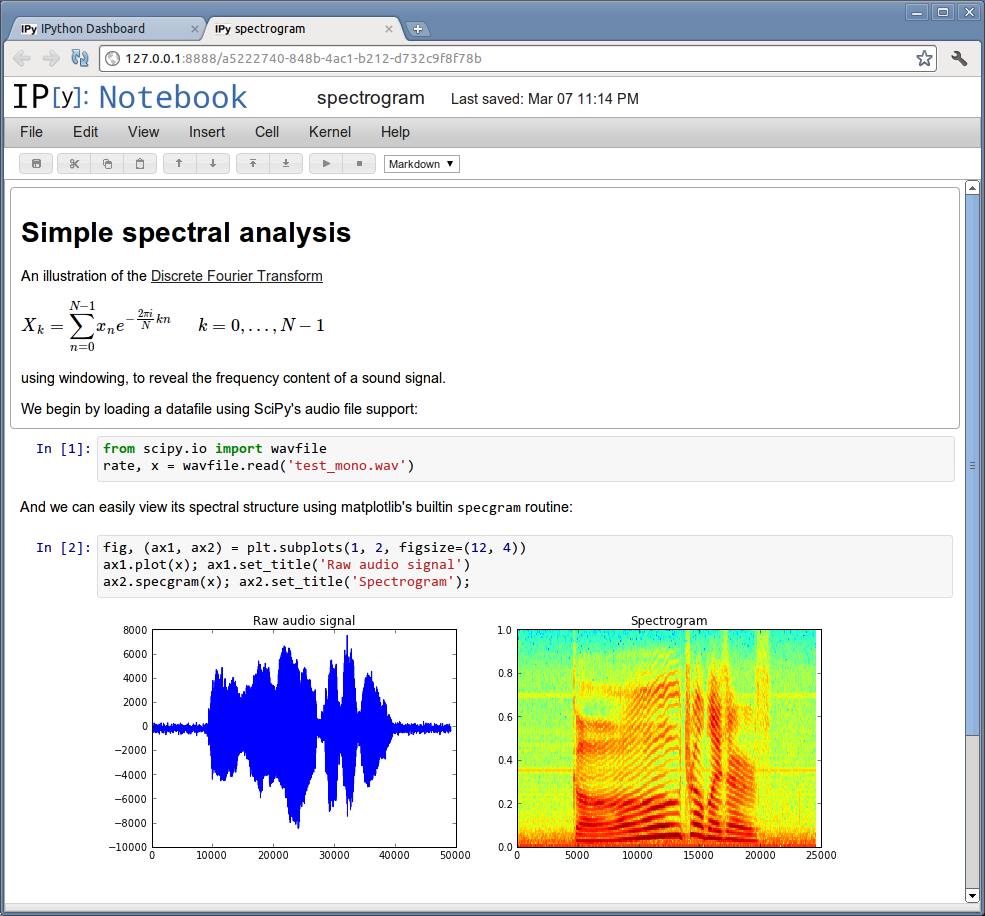
\includegraphics[width=3.2in]{fig/ipython-notebook-specgram.png}
\par\end{centering}

\caption{\label{fig:IPython-notebook}The web-based IPython Notebook combines
explanatory text, mathematics, multimedia, code and the results from
executing the code.}
\end{figure}



\section{Conclusion}\label{conclusion}

This is a large and complex problem that requires changing the educational
process for new scientists, the incentive models for promotions and
rewards, the publication system, and more.


\subsection{Changing culture}

Open{*}: software, access (Elsevier), education, review.

Internet: interactions for humans, code and data

\begin{itemize}
\item Open source software

\begin{itemize}
\item development akin to scientific culture
\item viable alternatives to proprietary software
\item tools and lessons for improving the scientific process: Github
\end{itemize}

\item Open access

\begin{itemize}
\item \url{thecostofknowledge.org}: Elsevier boycott
\item FRPAA House hearing on March 29th.
\end{itemize}

\item Open review
Ref \cite{10.3389/fncom.2012.00018}.

\item Open education

\begin{itemize}
\item MIT Open Courseware, Khan Academy\ldots
\item Stanford CS 221 in fall 2011: \textasciitilde{}160,000 students.
\item Spring 2012:

\begin{itemize}
\item Sebastian Thrun leaves Stanford: Udacity.
\item Stanford: Coursera.
\end{itemize}
\item MITx, TED-Ed\ldots
\end{itemize}
\end{itemize}

\subsection{Incentive models}

Science has become computational, but the incentive models of science
are single-mindedly focused on paper-oriented publications that completely
ignore the very existence of a computational process. Papers are accepted 

What role should journals play?

\begin{itemize}
\item Journals should mandate that upon paper \emph{approval} (but before
actual publication and with said publication being conditioned on
the author meeting this last condition), authors must expose their
version control system to the public, and that the publicly available
version can faithfully reproduce (within the limitations discussed
above) the published results. This public version then becomes available
for the scientific community not only for download, but also as a
starting point for further contribution and development.

\item supplemental material

\item peer review

\item new BioMed Central journal, Open Research Computation

 \item ongoing thematic series in Source Code for Biology and Medicine.
\cite{neylon2012changing}

\end{itemize}

How will all this impact scientists?

\begin{itemize}

\item funding
\item academic merit review

\end{itemize}

\subsection{Education and training}

\paragraph{ {\bf Workshops}}

\begin{itemize}

\item Software carpentry

\ldots basic training

\item Python

\ldots use of git

\end{itemize}

\paragraph{ {\bf Courses}}

\begin{itemize}

\item Josh

\item Randy

\item Titus

\end{itemize}


\section*{Acknowledgments}
We would like to thank
\begin{itemize}
\item members of the scientific Python community
\item scientist from various labs
\item Brian Granger
\item John Hunter
\item reviewers
\end{itemize}

\bibliographystyle{plain}
\bibliography{ipython}

\end{document}
